
\documentclass[12pt]{extarticle}
\usepackage[utf8]{inputenc}
\usepackage[english]{babel}
\usepackage[utf8]{inputenc}
\usepackage[english]{babel}
\usepackage[a4paper, total={7in, 9.5in}]{geometry}
\usepackage{tikz-cd}

 
\usepackage{amsthm, amssymb, amsmath, centernot, graphicx}
\usepackage{accents}
\DeclareMathAccent{\wtilde}{\mathord}{largesymbols}{"65}
\newcommand{\orb}[1]{\mathrm{Orb}(#1)}
\newcommand{\stab}[1]{\mathrm{Stab}(#1)}
\newcommand{\rp}{\mathbb{RP}}
\newcommand{\cp}{\mathbb{CP}}

\newcommand{\notimplies}{%
  \mathrel{{\ooalign{\hidewidth$\not\phantom{=}$\hidewidth\cr$\implies$}}}}
 
\renewcommand\qedsymbol{$\square$}
\newcommand{\cont}{$\boxtimes$}
\newcommand{\divides}{\mid}
\newcommand{\ndivides}{\centernot \mid}
\newcommand{\Z}{\mathbb{Z}}
\newcommand{\N}{\mathbb{N}}
\newcommand{\C}{\mathbb{C}}
\newcommand{\Zplus}{\mathbb{Z}^{+}}
\newcommand{\Primes}{\mathbb{P}}
\newcommand{\ball}[2]{B_{#1} \! \left(#2 \right)}
\newcommand{\Q}{\mathbb{Q}}
\newcommand{\R}{\mathbb{R}}
\newcommand{\Rplus}{\mathbb{R}^+}
\newcommand{\invI}[2]{#1^{-1} \left( #2 \right)}
\newcommand{\End}[1]{\text{End}\left( A \right)}
\newcommand{\legsym}[2]{\left(\frac{#1}{#2} \right)}
\renewcommand{\mod}[3]{\: #1 \equiv #2 \: \mathrm{mod} \: #3 \:}
\newcommand{\nmod}[3]{\: #1 \centernot \equiv #2 \: mod \: #3 \:}
\newcommand{\ndiv}{\hspace{-4pt}\not \divides \hspace{2pt}}
\newcommand{\finfield}[1]{\mathbb{F}_{#1}}
\newcommand{\finunits}[1]{\mathbb{F}_{#1}^{\times}}
\newcommand{\ord}[1]{\mathrm{ord}\! \left(#1 \right)}
\newcommand{\quadfield}[1]{\Q \small(\sqrt{#1} \small)}
\newcommand{\vspan}[1]{\mathrm{span}\! \left\{#1 \right\}}
\newcommand{\galgroup}[1]{Gal \small(#1 \small)}
\newcommand{\sm}{\! \setminus \!}
\newcommand{\topo}{\mathcal{T}}
\newcommand{\base}{\mathcal{B}}
\renewcommand{\bf}[1]{\mathbf{#1}}
\renewcommand{\Im}[1]{\mathrm{Im} \: #1}
\renewcommand{\empty}{\varnothing}
\newcommand{\id}{\mathrm{id}}
\newcommand{\Hom}[2]{\mathrm{Hom}\left( #1, #2 \right)}
\newcommand{\Tor}[4]{\mathrm{Tor}^{#1}_{#2} \left( #3, #4 \right)}

\renewcommand{\theenumi}{(\alph{enumi})}

\newcommand{\atitle}[1]{\title{% 
	\large \textbf{Mathematics GU4053 Algebraic Topology
	\\ Assignment \# #1} \vspace{-2ex}}
\author{Benjamin Church }
\maketitle}

\newcommand{\hook}{\hookrightarrow}


\theoremstyle{remark}
\newtheorem*{remark}{Remark}

\theoremstyle{definition}
\newtheorem{theorem}{Theorem}[section]
\newtheorem{lemma}[theorem]{Lemma}
\newtheorem{proposition}[theorem]{Proposition}
\newtheorem{corollary}[theorem]{Corollary}
\newtheorem{example}[theorem]{Example}


\newenvironment{definition}[1][Definition:]{\begin{trivlist}
\item[\hskip \labelsep {\bfseries #1}]}{\end{trivlist}}

\usepackage{subcaption}
\usepackage{float}
\floatplacement{figure}{H}

\begin{document}
\atitle{5}

Note. My order of path concatenation follows Hatcher,
\[\gamma * \delta(x) = \begin{cases}
\gamma(2x) & x \le \tfrac{1}{2} \\
\delta(2x - 1) & x \ge \tfrac{1}{2}
\end{cases}\]
 
\section*{Problem 1.}
Let $f : X \to Y$ and $g : Y \to Z$ be fibrations. Given any space $A$, a map $p : A \to X$ and a homotopy $h : A \times I \to Z$ consider the diagram,
\begin{center}
\begin{tikzcd}[column sep = huge, row sep = huge]
X \arrow[r, "f"] & Y \arrow[r, "g"] & Z \\
A \arrow[u, "p"] \arrow[ur, "f \circ p"] \arrow[rr, hook] & & A \times I \arrow[u, "h"] \arrow[ul, dashed, "\tilde{h}"]
\end{tikzcd}
\end{center} 
Because $g$ is a fibration, there exists a lift $\tilde{h} : A \times I \to Y$ of $h$ matching $f \circ p$ such that the diagram commutes. Now, rewrite the commutative diagram as,
\begin{center}
\begin{tikzcd}[column sep = huge, row sep = huge]
X \arrow[r, "f"] & Y \arrow[r, "g"] & Z \\
A \arrow[u, "p"]  \arrow[r, hook] & A \times I  \arrow[ur, "h"] \arrow[u, "\tilde{h}"] \arrow[ul, dashed, "\tilde{\tilde{h}}"] &
\end{tikzcd}
\end{center} 
which gives a lift $\tilde{\tilde{h}}$ of $\tilde{h}$ at $p$ because $f$ is a fibration. Therefore, there is a map $\tilde{\tilde{h}} : A \times I \to X$ which makes the diagram commute. That is, $\tilde{\tilde{h}}(a, 0) = p(a)$ and $g \circ f \circ \tilde{\tilde{h}} = g \circ \tilde{h} = h$. Thus, $g \circ f$ is a fibration.
\bigskip \\
Likewise, let $f : X \to Y$ and $g : Y \to Z$ be cofibrations. Given any space $A$, a map $p : Z \to A$ and a homotopy $h : X \times I \to A$ consider the diagram,
\begin{center}
\begin{tikzcd}[column sep = large, row sep = large]
X \arrow[rr, "f"] \arrow[dd, hook] & & Y \arrow[dl, "p \circ g"] \arrow[r, "g"] \arrow[dd, hook] & Z \arrow[dd, hook] \arrow[lld, bend left = 20, crossing over, "p"] \\
& A & & \\
X \times I \arrow[ru, "h"] \arrow[rr, "f \times \id_I"] & & Y \times I \arrow[r, "g \times \id_I"] \arrow[ul, dashed, "\tilde{h}"] & Z \times I
\end{tikzcd}
\end{center} 
Because $f$ is a cofibration, there exists an extension $\tilde{h} : Y \times I \to A$ of $h$ lifting to $p \circ g$ such that the diagram commutes. Now, rewrite the commutative diagram as,
\begin{center}
\begin{tikzcd}[column sep = large, row sep = large]
X \arrow[r, "f"] \arrow[dd, hook] & Y \arrow[rr, "g"] \arrow[dd, hook] & & Z \arrow[dd, hook] \arrow[dl, "p"] \\
& & A & \\
X \times I \arrow[r, "f \times \id_I"] & Y \times I \arrow[ur, "\tilde{h}"] \arrow[rr, "g \times \id_I"] & & Z \times I \arrow[ul, dashed, "\tilde{\tilde{h}}"]
\end{tikzcd}
\end{center} 
which gives an extension $\tilde{\tilde{h}}$ of $\tilde{h}$ lifting $p$ because $f$ is a cofibration. Therefore, there is a map $\tilde{\tilde{h}} : Z \times I \to A$ which makes the diagram commute. Thus, $g \circ f$ is a cofibration.

\section*{Problem 2.}

Let $f : X \to Y = \{ * \}$ be a continuous (constant map). Given a map $g : A \to X$ and a homotopy $h : A \times I \to Y$. However, $h$ must be a constant map so we should take $\tilde{h} : A \times I \to X$ given by $\tilde{h}(x, t) = g(x)$. Then, $f \circ \tilde{h} = h$ because both are constant maps. Also, $\tilde{h}(x, 0) = g(x)$ by construction. Thus, the following diagram commutes,
\begin{center}
\begin{tikzcd}[column sep = huge, row sep = huge]
X \arrow[r, "f"] & Y \\
A \arrow[u, "p"]  \arrow[r, hook] & A \times I \arrow[u, "h"] \arrow[ul, dashed, "\tilde{h}"]
\end{tikzcd}
\end{center} 
which means that $f$ is a fibration.

\section*{Problem 3.}

Let $p : E \to B$ be a continuous map and let $\pi : E^I \to N_p$ be the map $\pi(\gamma) = (\gamma(0), p \circ \gamma)$. Suppose there exists a section $s : N_p \to E^I$ such that $\pi \circ s = \id_{N_p}$. Now, for any topological space $Z$ with a map $f : Z \to E$ and homotopy $h : Z \times I \to B$ such that the following diagram commutes,
\begin{center}
\begin{tikzcd}[column sep = huge, row sep = huge]
Z \arrow[drr, "f", bend left] \arrow[rd, dashed, "m"] \arrow[ddr, "\hat{h}", bend right] & & E^I \arrow[d, "ev_0"] & \\
& N_p \arrow[r] \arrow[ur, "s", crossing over] \arrow[d] & E \arrow[d, "p"] & Z \arrow[lu, dashed, "u"] \arrow[d, hook] \arrow[l, "f"] \\
& B^I \arrow[r, "ev_0"] & B & Z \times I \arrow[l, "h"] \arrow[ul, "\tilde{h}", dashed]
\end{tikzcd}
\end{center}
Since we have a homotopy $h : Z \times I \to B$ by the adjunction relation there is a map $\hat{h} : Z \to B^I$. Because $N_p$ is the pullback of $B^I \to B \leftarrow Z \times I$ and there are maps $f$ and $\hat{h}$ from $Z$ which make the square commute, there exists a unique map $m = (f, \hat{h}) : Z \to N_p$ which makes the diagram commute. Then, define $u = s \circ m$. Finally, $u : Z \to E^I$ corresponds by the adjunction relation to a map $\hat{h} : Z \times I \to E$. We must check that this homotopy makes the rightmost square commute. Because $\pi \circ s = \id_{N_f}$ we know that $\pi \circ s(x, \gamma) = (s(x, \gamma)(0), p \circ s(x, \gamma)) = (x, \gamma)$. Therefore, $s(x, \gamma)(0) = x$ and $p \circ s(x, \gamma) = \gamma$. 
Now, 
\[\tilde{h}(z, 0) = (s \circ m)(z)(0) = s(m(z))(0) = s(f(z), \hat{h}(z)) (0) = f(z)\]
Likewise, 
\[p \circ \tilde{h}(z, t) = [p \circ s \circ m(z)](t) = [p  \circ s(f(z), \hat{h}(z))](t) = \hat{h}(z)(t) = h(z, t)\]
Therefore, the left square commutes so $p : E \to B$ is a fibration. \bigskip \\
Conversely, suppose that $p : E \to B$ is a fibration. We have maps $\pi_1 : N_p \to E$ such that $\pi_1(x, \gamma) = x$ and $\pi_2 : N_p \to B^I$ such that $\pi_2(x, \gamma) = \gamma$. By the adjunction relation, there is a map $h : N_p \times I \to B$ where $h(x, \gamma, t) = \pi_2(x, \gamma)(t) = \gamma(t)$. However, by the definition of $N_p$ we know that $p(x) = \gamma(0) = h(x, \gamma, 0)$ Therefore, the following diagram commutes,
\begin{center}
\begin{tikzcd}[column sep = huge, row sep = huge]
E^I \arrow[r, "ev_0"] & E  \arrow[r, "p"] & B \\
& N_p \arrow[u, "\pi_1"] \arrow[ul, "\hat{\tilde{h}}", dashed] \arrow[r, hook] & N_p \times I \arrow[u, "h"] \arrow[ul, "\hat{h}", dashed]
\end{tikzcd}
\end{center}   
Because $p$ is a fibration, there exists a map $\tilde{h} : N_p \times I \to E$ which makes the diagram commute. By the adjuction relation, this gives a map $\hat{\tilde{h}} : N_p \to E^I$. I claim that this is the section we are searching for. Consider,
\[ \pi \circ \hat{\tilde{h}}(x, \gamma) = (\hat{\tilde{h}}(x, \gamma)(0), p \circ \hat{\tilde{h}}(x, \gamma)) = (\tilde{h}(x, \gamma, 0), p \circ \hat{\tilde{h}}(x, \gamma)) \] 
However, the consider the loop,
\[ p \circ \hat{\tilde{h}}(x, \gamma)(t) = p \circ \tilde{h}(x, \gamma, t) = h(x, \gamma, t) = \gamma(t) \]
Also $\tilde{h} \circ \iota = \pi_1$ so $\tilde{h}(x, \gamma, 0) = \pi_1(x, \gamma) = x$. Therefore,
\[ \pi \circ \hat{\tilde{h}}(x, \gamma) = (\tilde{h}(x, \gamma, 0), p \circ \hat{\tilde{h}}(x, \gamma)) = (x, \gamma) \] 
Thus, $\pi \circ s = \id_{N_p}$ so $s$ is a section.

\section*{Problem 4.}

Let $p : \Delta^2 \to \Delta^1$ be the projection of a 2-simplex onto a side which is a 1-simplex. We will consider a 2-simplex as a right triangle for simplicity.
We will geometrically define the a map $g : \Delta^2 \times \Delta^1 \to \Delta^2$ such that $p \circ g(x, y) = y$ and $g(x, (p(x)) = x$.

\begin{center} 
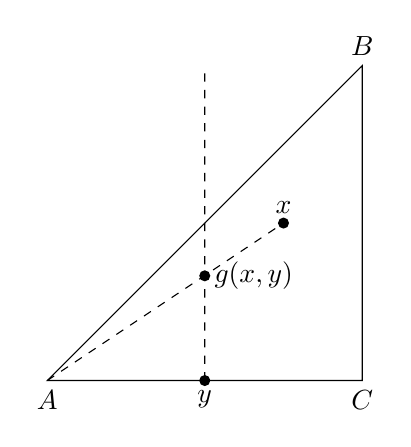
\begin{tikzpicture}
\fill
  (3, 2) circle (2pt) node[anchor=south]{$x$}
  (2, 0) circle (2pt) node[anchor=north]{$y$}
  (2, 1.33) circle (2pt) node[anchor=west]{$g(x,y)$};
\draw[dashed] 
  (0,0) -- (3, 2)
  (2, 0) -- (2, 4);
\draw
	(0,0) node[anchor=north]{$A$}
  -- (4,0) node[anchor=north]{$C$}
  -- (4,4) node[anchor=south]{$B$}
  -- cycle;
\end{tikzpicture}
\end{center}
Clearly, if $y = p(x)$ then $x$ lies on the perpendicular bisector of $AC$ at $y$ so $g(x, p(x)) = x$. Furthermore, $p(g(x,y)) = y$ because $g(x,y)$ lies directly above $y$ on the perpendicular bisector of $AC$ at $y$.
Given such a map, define the section $s : N_p \to  (\Delta^2)^I$ given by $s(x, \gamma) = g(x, \gamma(-))$. Then,
\[ \pi \circ s(x, \gamma) = \pi(g(x, \gamma(-)) = (g(x, \gamma(0)), p \circ g(x, \gamma(-))) \]
but $\gamma(0) = p(x)$ because $(x, \gamma) \in N_p$ and $g(x, p(x)) = x$ and $p \circ g(x, \gamma(-)) = \gamma$. Therefore,
\[ \pi \circ s(x, \gamma) = (g(x, \gamma(0)), p \circ g(x, \gamma(-))) = (x, \gamma) \]
so $\pi \circ s = \id_{N_p}$. Therefore, $s$ is a section of the map $\pi : E^I \to N_p$ so by the above problem $p : \Delta^2 \to \Delta^1$ is a fibration. However, $p$ cannot be a fiber bundle because the inverse image of the left endpoint is a line segment while the inverse image of the right endpoint is a sinlge point. Since the fibers are not homeomorphic the map cannot be a fiber bundle.  

\section*{Problem 5.}
Let $(X, x_0)$ and $(Y, y_0)$ be pointed spaces.
Consider the map $\Hom{\Sigma X}{Y} \to \Hom{X}{\Omega Y}$ which send maps,
\[ ((x \wedge t) \mapsto f(x \wedge t)) \mapsto (x \mapsto ( t \mapsto f(x \wedge t))) \] 
Since $x_0 \wedge t_0 = x_0 \sim t$ we must have $f(x_0 \wedge t) = y_0$ be constant. Thus, the function $f$ is taken to $x \mapsto ( t \mapsto f(x \wedge t))$ which has the property that $x_0 \mapsto (t \mapsto f(x_0 \wedge t) = f(x_0 \wedge t_0) = y-9$. Thus, $x_0 \mapsto e_0$ the basepoint of $\Omega Y$. Thus, this correspondence sends based maps to based maps. Furthermore, given a based map in $\Hom{X}{\Omega Y}$ written as $x \mapsto (t \mapsto f(x, t))$ for $f \in \Hom{X \times S^1}{Y}$, we know that $x_0 \mapsto e_0$ the constant map at $y_0$. Thus, $f(x_0, t) = y_0$. Furthermore, $x$ must map to a based map $S^1 \to Y$ so $f(x, t_0) = y_0$. Thus, $f$ is constant on $X \vee S^1$ so $f$ as a function on $X \times S^1$ decends to the quotient $X \wedge S^1 = X \times S^1 / X \vee S^1$. Thus, $f$ is in the image of the correspondence so the mapping is surjective. Furthermore, the correspondence is one-to-one because if $f(x, t) = g(x, t)$ then clearly  
$f(x \wedge t) = g(x \wedge t)$ because these are simply restriction maps. Thus, $\Hom{\Sigma X}{Y} \cong \Hom{X}{\Omega Y}$. It suffices to show that this correspondence descends to homotopy classes. This is clear because any homotopy $H : (X \wedge S^1) \times I \to Y$ is in correspondence to a homotopy $H : X \times I \to \Omega Y$ by exactly the same correspondence outlied above taken on each time slice. Thus, a homotopy between maps in one Hom space is equivalent to a homotopy between the corresponding maps in the other. Therefore, 
\[ \left< \Sigma X, Y \right> = \left<X, \Omega Y \right> \] 
\section*{Problem 6.}

Let $X$ be a CW complex equal to an increasing union of subcomplexes, 
\[ X_1 \subset X_2 \subset X_3 \subset X_4 \subset \cdots \quad \quad \text{and} \quad \quad X = \bigcup_{i = 1}^\infty X_i \]
such that each inclusion $X_i \hookrightarrow X_{i+1}$ is nullhomotopic. I claim that, picking a basepoint $\{x_0\}$, the complex $X = \lim\limits_{\rightarrow} X_i$ is the direct limit (colimit) of the system,
\begin{center}
\begin{tikzcd}
\{x_0\} \arrow[r, hook] & X_1 \arrow[r, hook] & X_2 \arrow[r, hook] & X_3 \arrow[r, hook] & X_4 \arrow[r, hook] & \cdots
\end{tikzcd}
\end{center} 
The projection functor $\pi : \mathbf{Top} \to \mathbf{hTop}$ maps topological spaces to themselves and maps maps to homotopy classes is cocontinuous so,  
\[\pi(X) = \pi(\lim\limits_{\rightarrow} X_i) \cong \lim\limits_{\rightarrow} \pi(X_i)\]
However, each inclusion map $\iota$ is nullhomotopic. Therefore, in $\mathbf{hTop}$ each of these maps is a constant map so the one point space satisfies the universal property of the limit. In particular, let $j_1 : X_i \to X = *$ be the universal cones. Take any other space, $A$ with maps $f_i : X_i \to A$ such that $f_{i} = f_{i + 1} \circ \iota_{i + 1}$. However, $\iota_{i + 1}$ is a constant map so $f_{i}$ must be constant. Moveover, $f_{i}$ and $f_{j}$ must have the same image because  $f_{i}(x) = f_{i + 1}(\iota_{i + 1}(x)$ and both are contant. Therefore, this entire system factors though $X = *$ via a map from $* \to \{f_{i}(x)\}$. Thus, the one point space is the direct limit of this system in $\mathbf{hTop}$. However, the original directed system in $\mathbf{Top}$ must project via $\pi$ down to this system in $\mathbf{hTop}$. Since colimits are unique, $X$ is isomorphic to $*$ in $\mathrm{hTop}$ which implies that $X$ is homotopy equivalent to $*$ i.e. $X$ is contractable.     

\section*{Problem 7.}

Consider the pointed space $(X, x_0)$ and the suspension $\Sigma X \cong X \times I / (X \times \{0\} \cup X \times \{1\} \cup \{x_0\} \times I) $. Consider the homotopy, $X \times I \to \Sigma X$ defined by $h(x, t) = (x, t/2)$. Then, $h(x, 0) = (x, 0)$ but $(x_1, 0) \sim (x_2, 0)$ so $h(x, 0)$ is constant. Also, $h(x, 1) = (x, 1/2) = \iota(x)$. Therefore, $\iota : X \hookrightarrow \Sigma X$ is nullhomotopic. 

\section*{Problem 8.}

Let $X$ be a pointed CW complex. The infinite suspension of $X$ is given by,
\[ \Sigma^\infty (X) = \bigcup_{i = 1}^\infty \Sigma^i(X) \]
Choosing a basepoint $x_0$, by problem $7$, the inclusion maps in the following chain are nullhomotopic,
\begin{center}
\begin{tikzcd}
\{x_0\} \arrow[r, hook] & X \arrow[r, hook] & \Sigma X \arrow[r, hook] & \Sigma^2 X\arrow[r, hook] & \Sigma^3 X \arrow[r, hook] & \Sigma^4 X \arrow[r, hook] & \Sigma^5 X \arrow[r, hook] & \Sigma^6 X \arrow[r, hook] & \cdots
\end{tikzcd}
\end{center} 
which, by problem $7$, implies that the total complex $\Sigma^\infty(X)$ is contractable.
\end{document}
